\section{Theorie}
Um Informationen mit Hilfe von elektromagnetischen Wellen übertragen zu können werden Verfahren benötigt um diesen Wellen
Informationen aufprägen zu können. Solche Verfahren werden Modulationsverfahren genannt, dass Rückgewinnen der Informationen aus der 
modulierten Welle nennt man Demodulation.

Die Hochfrequenztechnik kennt eine Reihe von Modulationsverfahren, welche unter Ausnutzung einer periodischen Änderung von 
Amplitude, Frequenz oder Phase einer Trägerwelle dieser Informationen aufprägen.

\subsection{Amplitudenmodulation}
Die einfachste Form der Amplitudenmodulation lässt die Amplitude einer hochfrequenten Trägerwelle $U_T(t)$ im Rythmus einer niederfrequenten Modulationswelle $U_M(t)$ varrieren. Die Trägerwelle besitzt die Frequenz $\omega_T$ und die Modulationswelle die
Frequenz $\omega_M$.

Die amplitudenmodulierte Schwingung soll dann eine mit $\omega_M$ varrierende Amplitude

\begin{equation}
U_{3}(t) = U_T (1 + m \cos( \omega_M t))\cos(\omega_T t)
\label{eq:AmMod}
\end{equation} 

besitzen. Wobei $m = \gamma U_M$ den  Modulationsgrad der Schwinung beschreibt.

\begin{figure}
	\centering
	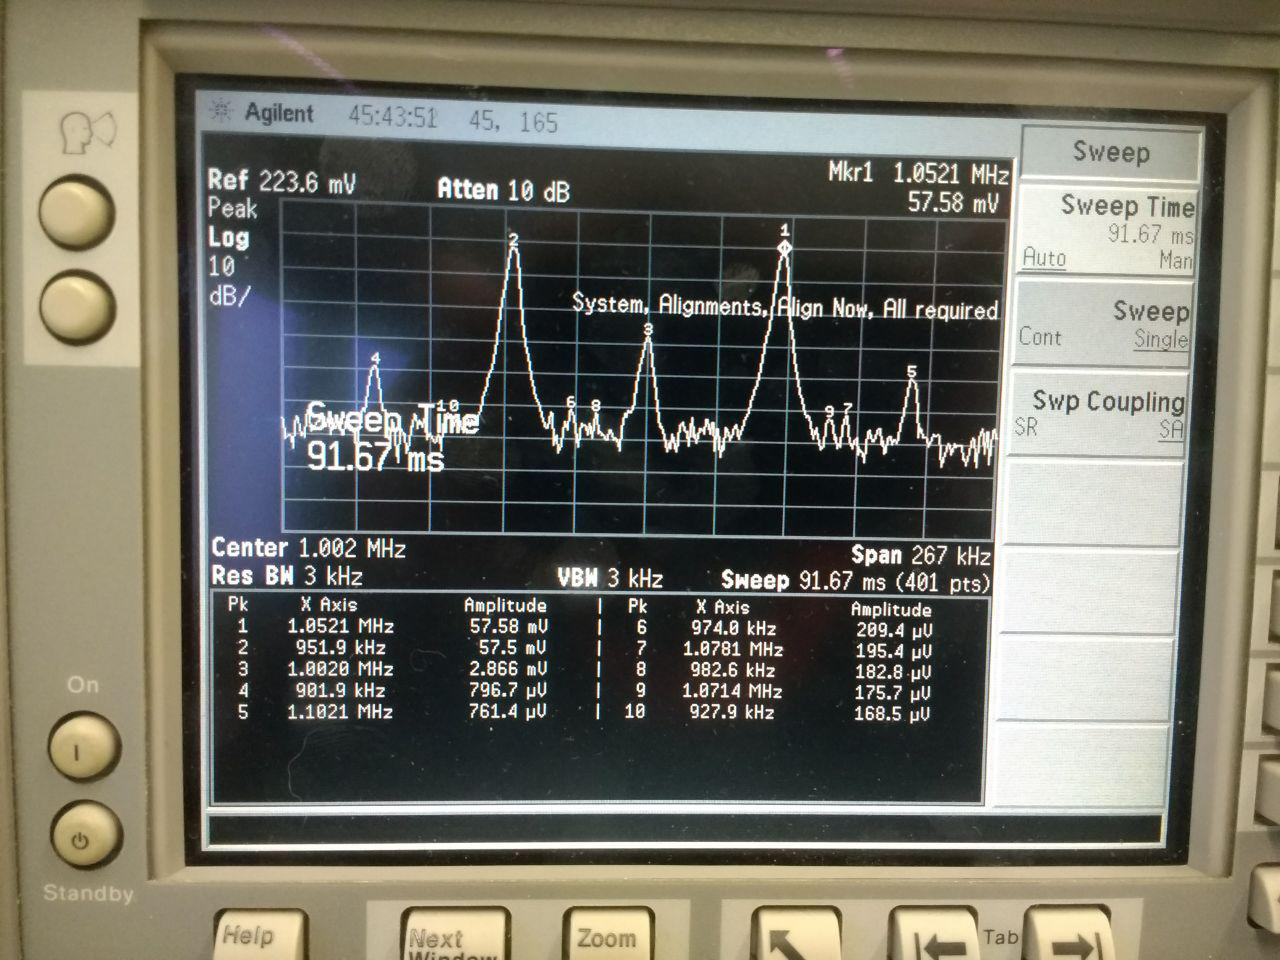
\includegraphics[width=\textwidth]{img/Aufgabenteil_b.jpg}
	\caption{Zeitabhängigkeit der Signalspannung eines Amplitudenmodulierten Signals}
\end{figure}

Wird durch geeignete Umformung oder Fouriertransformation das Frequenzspektrum der Schwinung analysiert

\begin{equation}
U_{3}(t) = U_T ( \cos(\omega_T t) + \frac{1}{2}m\cos(\omega_T + \omega_M)t + \frac{1}{2}m\cos(\omega_T - \omega_M)t)
\label{eq:FreqAmMod}
\end{equation}

fällt auf, dass in diesem einfachen Fall bereits drei Frequenzen beteiligt sind.

\begin{figure}
	\centering
	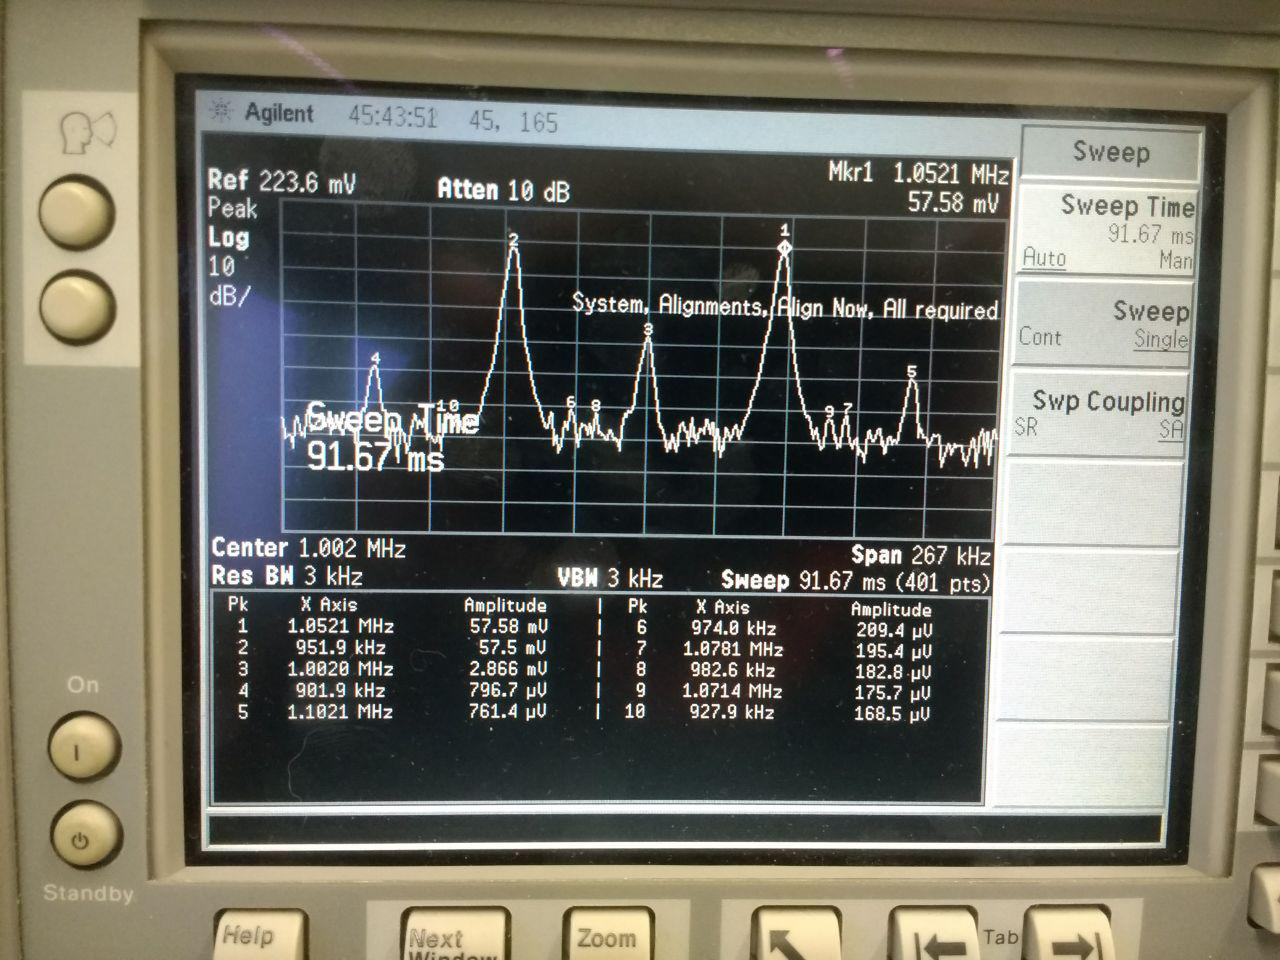
\includegraphics[width=\textwidth]{img/Aufgabenteil_b.jpg}
	\caption{Frequenzspektrum einer Amplitudenmodulierten Schwingung}
\end{figure}

Die Frequenz bei $\omega_T$ nennt man Trägerfrequenz, diese Trägt keine Information und stellt einen dissipativen Anteil dar, welcher in der Praxis unerwünscht ist. Auch beschreiben die beiden Seitenbänder bei $\omega_T - \omega_M$ und $\omega_T + \omega_M$ die gleichen Informationen. Somit ist es üblich eines der Beiden Seitenbänder durch geeignete Filter zu unterdrücken.
Wird die Trägerfrequenz und ein Seitenband unterdrückt wird auch von Einseitenbandmodulation mit Trägerunterdrückung gesprochen.
Die großen Nachteile der Amplitudenmodulation besteht in ihrer geringen Störsicherheit und geringen Verzerrungsfreiheit.

\subsection{Frequenzmodulation}
Anders als bei der Amplitudenmodulation wird bei der Frequenzmodulation die momentane Schwingungsfrequenz im Rythmus des Modulationssignales varriert.

\begin{equation}
U(t)= U\sin(\omega_T t + m \frac{\omega_T}{\omega_M} \cos(\omega_M t))
\label{eq:FreqMod}
\end{equation}

Durch Differentation des Arguments des Sinues ergibt sich die Momentanfrequenz

\begin{equation}
f(t) = \frac{\omega_T}{2\pi}(1-m\sin(\omega_M t))
\label{eq:momFreq}
\end{equation}

der Schwingung. Wobei m wieder den Modulationsgrad und $\frac{m\omega_T}{2|pi}$ den Frequenzhub geschreibt. Der Frequenzhub ist es Maß dafür, wie Stark die Schwinungsfrequenz varriert. Im folgenden ist eine Schmalbald-Frequenzmoduation zu sehen, welche sich durch

\begin{equation}
m\frac{\omega_T}{\omega_M} << 1
\end{equation}

auszeichnet.

\begin{figure}
	\centering
	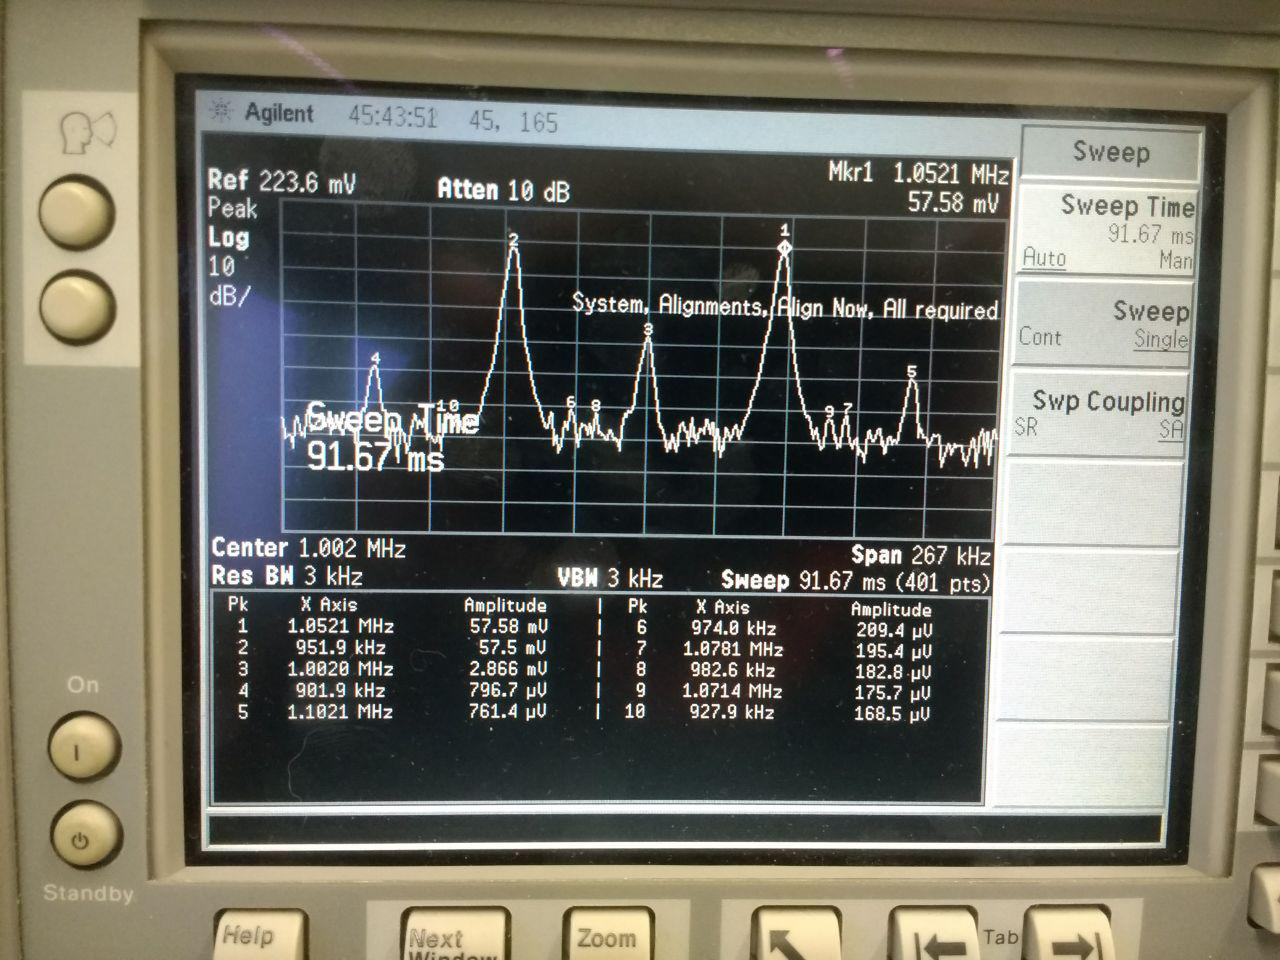
\includegraphics[width=\textwidth]{img/Aufgabenteil_b.jpg}
	\caption{Zeitlicher Verauf einer frequenzmodulierten Schwindung}
\end{figure}

Durch geeignete Umformung oder Fouriertransfromation ist ersichtlich, dass auch das Frequenzspektrum der Frequenzmodulation sich aus drei
Frequenzen zusammensetzt.

\begin{equation}
U(t) = U(\sin(\omega_T t) + \frac{m\omega_T}{2\omega_M}\cos(\omega_T + \omega_M) t \frac{m\omega_T}{2\omega_M}\cos(\omega_T - \omega_M) t)
\label{eq:FreqFreqMod}
\end{equation}

Es fällt auf, dass die beiden Seitenbänder im Fall der Frequenzmodulation um $\frac{\pi}{2}$ gegebüber der Trägerschwingung vershoben sind. Es ist anzumerken, dass das o.g. Frequenzspektrum nur im Fall der schwach frequenzmodulierten Schwingung

\begin{equation}
\frac{m\omega_T}{\omega_M} << 1
\end{equation}

gültigkeit besitzt. Im Fall der starken Frequenzmodulation

\begin{equation}
m\omega_T \approx \omega_M
\end{equation}

besitzt das Frequenzspektrum eine komplexere Darstellung der Form

\begin{equation}
U(t) = U \sum_{n=-\inf}^{+\inf} J_{n}(\frac{m\omega_T}{\omega_M})\sin(\omega_T + n\omega_M)t 
\end{equation}

wobei $J_n$ die Besselsche Funktion n-ter Ordnung ist. Es zeigt sich, dass für hohe Modulationsgrade das Frequenzspektrum im prinzip bis zu beliebig hohen Frequenzen reicht. Es reicht jedoch in der Praxis nur Frequenzen in der Nähe der Trägerfrequenz zu berücksichtigen, da

\begin{equation}
J_{\pm n}(x) \approx \frac{1}{\sqrt{2\pi n}}(\frac{ex}{2n})^n
\end{equation}

mit wachsender Ordnungszahl n und $x <= 1$ schnell gegen null geht.

\subsection{Modulationsschaltungen}
Um die Amplitude einer Trägerschwingung zu modulieren \ref{eq:AmMod} wird ein Bauteil benötigt, welches das Produkt aus zwei Eingagspannungen bilden kann. Grundsätzlich ist das mit jedem Bauteil möglich, welches eine nichtlineare Kennlinie besitzt.
Eine solche Schaltung kann z.B. mit Hilfe einer Diode gemäß \ref{abb:simpleMod} realisiert werden.

\begin{figure}
	\centering
	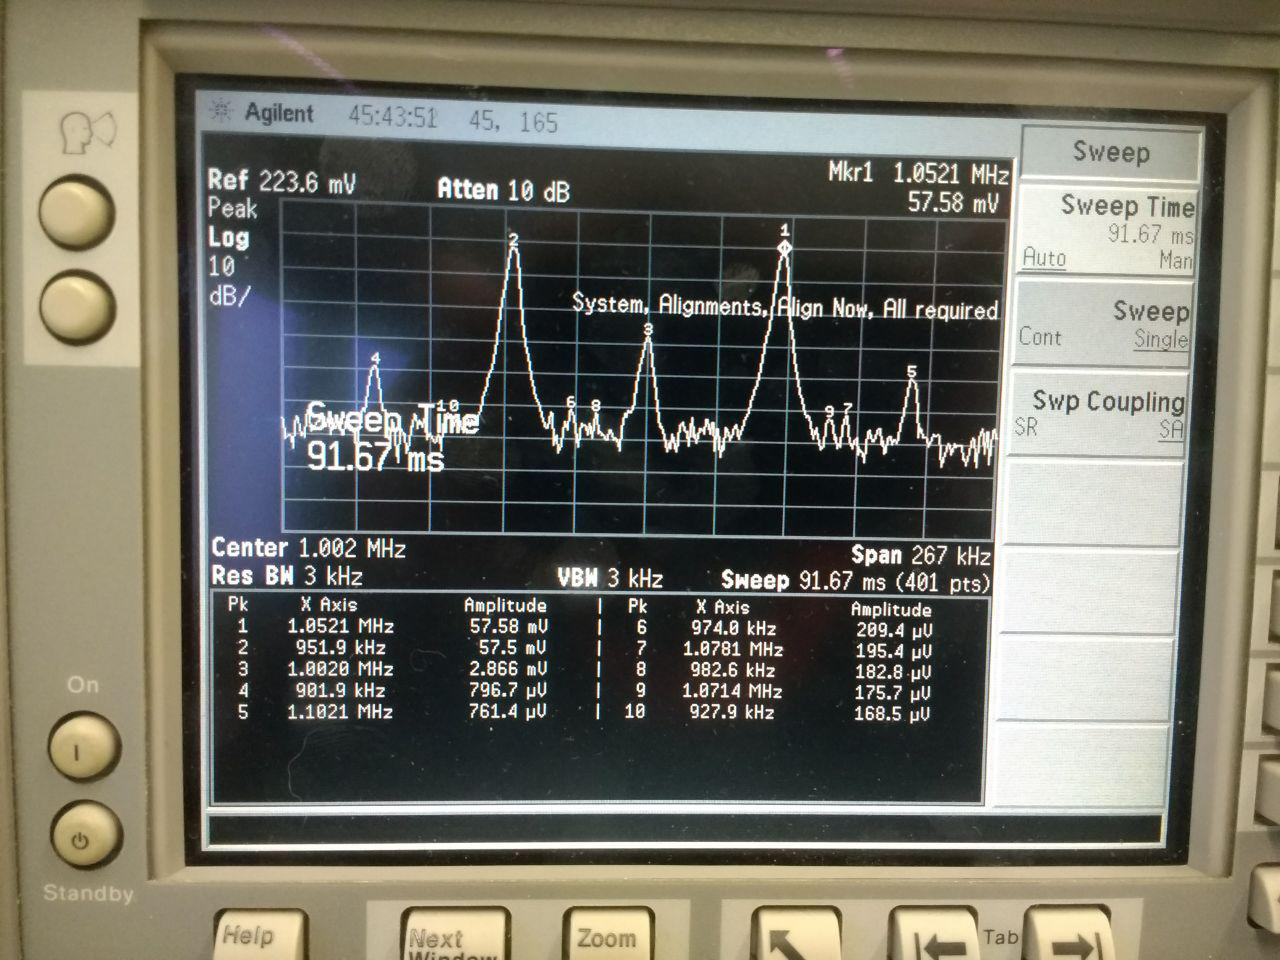
\includegraphics[width=\textwidth]{img/Aufgabenteil_b.jpg}
	\caption{Primitive Modulatorschaltung}
	\label{abb:simpleMod}
\end{figure}

Wird die Summe von Träger- und Modulatorspannung für die Spannung in die Potzenreihenentwicklung der Diodenkennlinie eingesetzt

\begin{equation}
I(U_T + U_M) = a_0 + a_1(U_T + U_M) + a_2(U_T^2 + U_M^2) + 2a_2 U_T U_M + ...
\end{equation}

liefert das vierte Reihenglied das geforderte Produkt. Es fällt auf das zusätzliche Störterme aufreten, dessen Frequenzen  $\omega_M, 2\omega_M und 2\omega_T$ allerdings weit außerhalb des zu übertragenden Frequenzbandes $\omega_T - \omega_M$ bis $\omega_T + \omega_M$ liegen, sodass diese mit einem geeigneten Bandfilter unterdückt werden können.
Durch das Erzeugen der vielen nicht genutzten Frequenzen ist so eine Schaltung sehr unökonomisch. Es ist wünschenswert das die Störenden Frequenzanteile erst garnicht erzeugt werden.

\subsubsection{Der Ringmodulator}
Der Ringmodulator besteht, wie der Name bereits andeutet, aus einem Ring von vier zusammengeschaltet Dioden.

\begin{figure}
	\centering
	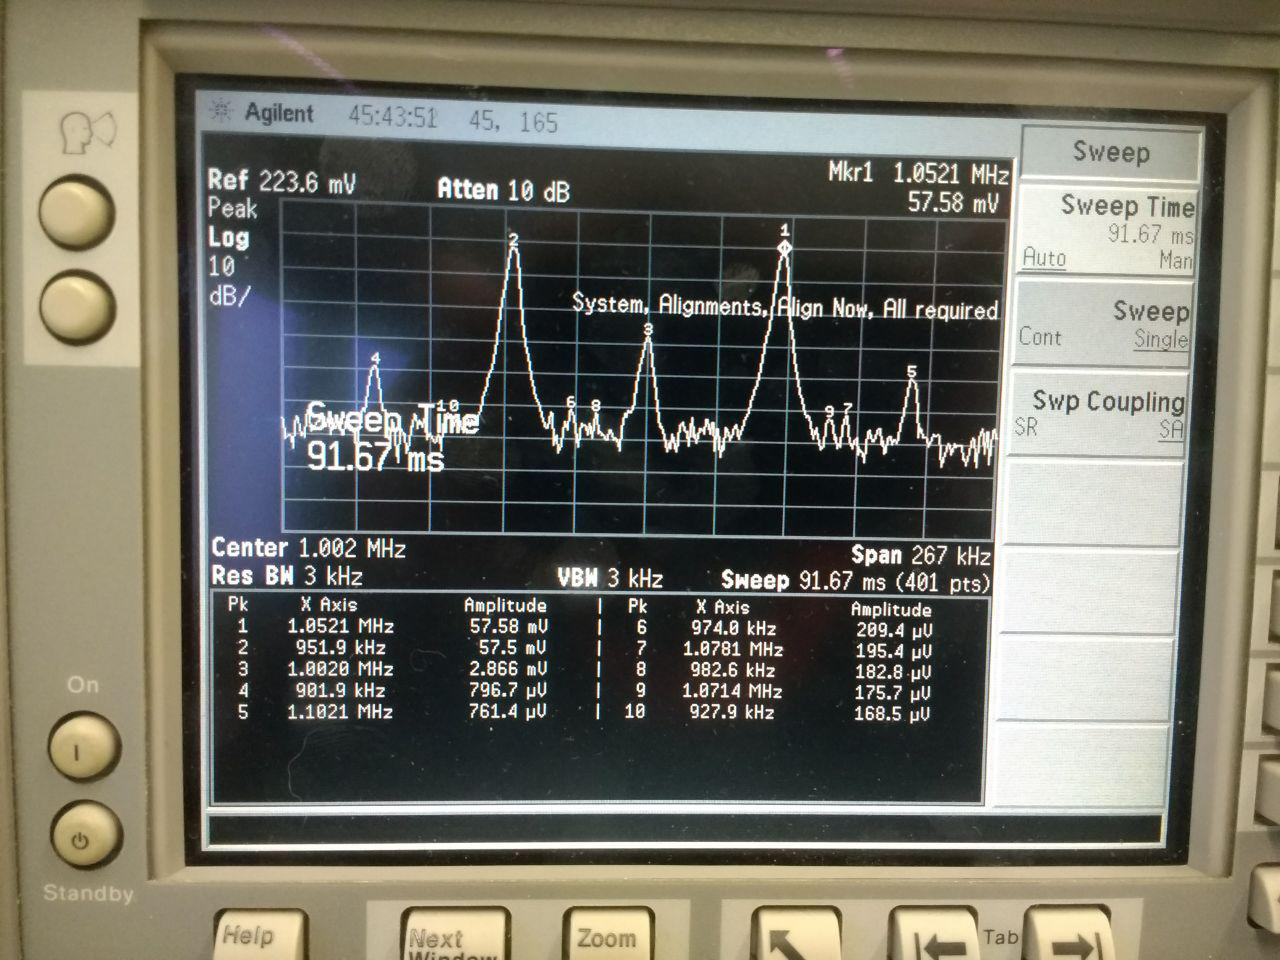
\includegraphics[width=\textwidth]{img/Aufgabenteil_b.jpg}
	\caption{Primitive Modulatorschaltung}
	\label{abb:ringMod}
\end{figure}

Diese Schaltung ist in der Lage das Produkt von Träger und Modulationssignal zu bilden ohne störende parasitäre Frequenzanteile zu erzeugen. Die abgenommene Spannung ist direkt proportional zum Produkt der Eingangsspannungen.

\begin{equation}
U_R(t) = \gamma U_M(t) \cdot U_T(t)
\label{eq:ringMod}
\end{equation}

Es ist anzumerken, dass $\gamma$ die Einehit $\frac{1}{V}$ besitzt. Es ist direkt ersichtich, dass der Ringmodulator die Trägerabstrahlung unterdrückt. Werden zwei Cosinus-Signale für $U_T$ und $U_M$ mit den Frequenzen $\omega_T$ und $\omega_M$ in \ref{eq:ringMod} eingesetzt folgt

\begin{equation}
U_R(t) = \gamma U_T U_M \frac{1}{2}\cos((\omega_T + \omega_M)t + \phi) + \gamma U_T U_M \frac{1}{2} \cos((\omega_T - \omega_M)t - \phi)
\end{equation}
.

Wie bereits angesprochen fehlt in diesem Frequenzspektrum der Trägeranteil $\omega_T$.

\subsubsection{Frequenzmodulator mit geringem Frequenzhub}
\subsection{Demodulationsschaltungen}